%页面设置
\documentclass[a4paper]{article}
\usepackage[top=1in,bottom=1in,left=1in,right=1in]{geometry}
%\usepackage[utf8]{inputenc}
\usepackage{titlesec} %标题位置,有center,raggedleft,raggedright三个选项
\linespread{1.3}\selectfont
%本地化
\usepackage{fontspec}
\setmainfont{SimSun}
\XeTeXlinebreaklocale "zh"
\XeTeXlinebreakskip = 0pt plus 1pt minus 0.1pt
%数学
\usepackage{amsmath}
\makeatletter
\def\verbatim@font{} %如果使用roman字体族,将sffamily改成rmfamily
\makeatother
%文档
\begin{document}
\title{现代控制理论}
\author{船海 闫鹏 201430110059}
\date{}
\maketitle
\noindent
\section*{第一题}
\mbox{已知 }$ A=\left(\begin{array}{ccc} 1 & 0 & -1\\ 0 & -2 & 0\\ -1 & 0 & 2 \end{array}\right) $,
$ B=\left(\begin{array}{c} 0\\ 0\\ 1 \end{array}\right) $,  $ C=\left(\begin{array}{ccc} 1 & 0 & 0 \end{array}\right)$. \\
$ G(s)=C(sI-A)^{-1}B $,\mbox{且}
$ (sI-A)=\left(\begin{array}{ccc} s - 1 & 0 & 1\\ 0 & s + 2 & 0\\ 1 & 0 & s - 2 \end{array}\right) $ \\
\mbox{通过初等函数法求逆矩阵} \\
\begin{displaymath}
\left(\begin{array}{cccccc} s - 1 & 0 & 1 & 1 & 0 & 0\\ 0 & s + 2 & 0 & 0 & 1 & 0\\ 1 & 0 & s - 2 & 0 & 0 & 1 \end{array}\right) = \left(\begin{array}{cccccc} 1 & 0 & 0 & \frac{s - 2}{s^2 - 3\, s + 1} & 0 & -\frac{1}{s^2 - 3\, s + 1}\\ 0 & 1 & 0 & 0 & \frac{1}{s + 2} & 0\\ 0 & 0 & 1 & -\frac{1}{s^2 - 3\, s + 1} & 0 & \frac{s - 1}{s^2 - 3\, s + 1} \end{array}\right)
\end{displaymath} \\
\mbox{故逆矩阵 }$(sI-A)^{-1}= \left(\begin{array}{ccc} \frac{s - 2}{s^2 - 3\, s + 1} & 0 & -\frac{1}{s^2 - 3\, s + 1}\\ 0 & \frac{1}{s + 2} & 0\\ -\frac{1}{s^2 - 3\, s + 1} & 0 & \frac{s - 1}{s^2 - 3\, s + 1} \end{array}\right) $ \\
$$ G(s)=C(sI-A)^{-1}B = \left(\begin{array}{ccc} 1 & 0 & 0 \end{array}\right) \left(\begin{array}{ccc} \frac{s - 2}{s^2 - 3\, s + 1} & 0 & -\frac{1}{s^2 - 3\, s + 1}\\ 0 & \frac{1}{s + 2} & 0\\ -\frac{1}{s^2 - 3\, s + 1} & 0 & \frac{s - 1}{s^2 - 3\, s + 1} \end{array}\right) \left(\begin{array}{c} 0\\ 0\\ 1 \end{array}\right) =   \frac{s + 2}{ - s^3 + s^2 + 5\, s - 2} $$ \\
\mbox{上下通分可得 } \\
$$G(s)= \frac{-1}{ s^2 -3s +1} $$
\begin{verbatim}[matlab]
[num ,den]=ss2tf(A,B,C,D)
num =
     0     0    -1    -2
den =
     1    -1    -5     2
\end{verbatim} 
\section*{第二题} 
先求状态转移矩阵\\
\mbox{系统特征方程式为 }$\left|{\lambda}I-A \right|=\left|\begin{array}{ccc} t - 1 & 0 & 1\\ 0 & t + 2 & 0\\ 1 & 0 & t - 2 \end{array}\right|=t^3 - t^2 - 5\, t + 2=0 $ \\
\mbox{可解系统特征值为 }$\lambda= -2,0.3820,2.6180$,为互异特征值。因此可以代入$({\lambda}I-A){\zeta}=0 $,求出特征向量,将矩阵A化为对角阵。\mbox{令 }$\zeta=\left(\begin{array}{ccc} x1 \\ x2 \\x3 \end{array}\right) $ \\
\mbox{当 }$\zeta=-2$时,$\left(\left[\begin{array}{ccc} -2 & 0 & 0 \\ 0 & -2 & 0 \\ 0 & 0 & -2 \end{array}\right]-\left[\begin{array}{ccc} 1 & 0 & -1 \\ 0 & -2 & 0 \\ -1 & 0 & 2 \end{array}\right]\right)\left[\begin{array}{ccc} x_{1} \\ x_{2}  \\ x_{3} \end{array}\right]=0$得 \\
\begin{align*}
-3x_1+x_3 &= 0 \\
x_1-4x_3 &= 0
\end{align*}
得$x_1=x_3=0,x_2=1$ \\
当$\lambda=0.382$时,$ \left(\left[\begin{array}{ccc} 0.382 & 0 & 0\\ 0 & 0.382 & 0\\ 0 & 0 & 0.382 \end{array}\right]-\left[\begin{array}{ccc} 1 & 0 & -1\\ 0 & -2 & 0\\ -1 & 0 & 2 \end{array}\right]\right)\left[\begin{array}{ccc} x_{1} \\ x_{2}  \\ x_{3} \end{array}\right]=0 $得\\
\begin{align*}
0.618x_1+x_3 &= 0 \\
x_2 &= 0 \\
x_1-1.618x_3 &=0
\end{align*}
\mbox{令 }$x_1=1$,\mbox{得 }$x_3=-0.618$ \\
\mbox{当 }$ \lambda=2.618$\mbox{时},$ \left(\left[\begin{array}{ccc} 2.618 & 0 & 0\\ 0 & 2.618 & 0\\ 0 & 0 & 2.618 \end{array}\right]-\left(\begin{array}{ccc} 1 & 0 & -1\\ 0 & -2 & 0\\ -1 & 0 & 2 \end{array}\right)\right)\left[\begin{array}{ccc} x_{1} \\ x_{2}  \\ x_{3} \end{array}\right]=0 $得\\
\begin{align*}
1.618x_1+x_3 &= 0 \\
x_2 &= 0 \\
x_1+0.618x_3 &= 0
\end{align*}
\mbox{令 }$x_1=1$,得$x_3=-1.618$ \\
\mbox{得到矩阵}$ \left[\begin{array}{ccc} 0 & 1 & 1 \\ 1 & 0 & 0 \\ 0 & -0.618 & -1.618\end{array}\right] $,经过施密特正交化可得最后特征矩阵 \\
$$ P=\left(\begin{array}{ccc} 0 & -0.85065 & -0.52573\\ 1.0 & 0 & 0\\ 0 & -0.52573 & 0.85065 \end{array}\right),
P^{-1}=\left(\begin{array}{ccc} 0 & 1.0 & 0\\ -0.85065 & 0 & -0.52573\\ -0.52573 & 0 & 0.85065 \end{array}\right) $$ \\
\mbox{对角阵 }$ \Lambda=PAP^{-1}= \left(\begin{array}{ccc} -2.0 & 0 & 0\\ 0 & 0.38197 & 0\\ 0 & 0 & 2.618 \end{array}\right) $ \\
通过线性变换法可求 \\
$$ \Phi(t)=
e^{At}=P^{-1}e^{{\Lambda}t}P= \left(\begin{array}{ccc} 0.27639\, \mathrm{e}^{2.618\, t} + 0.72361\, \mathrm{e}^{0.38197\, t} & 0 & 0.44721\, \mathrm{e}^{0.38197\, t} - 0.44721\, \mathrm{e}^{2.618\, t}\\ 0 & \mathrm{e}^{- 2.0\, t} & 0\\ 0.44721\, \mathrm{e}^{0.38197\, t} - 0.44721\, \mathrm{e}^{2.618\, t} & 0 & 0.72361\, \mathrm{e}^{2.618\, t} + 0.27639\, \mathrm{e}^{0.38197\, t} \end{array}\right) $$ \\
\mbox{故 }
\begin{align*}
\Phi(t)x(0) &= \left(\begin{array}{c} 1.1708\, \mathrm{e}^{0.38197\, t} - 0.17082\, \mathrm{e}^{2.618\, t}\\ 2\, \mathrm{e}^{- 2.0\, t}\\ 0.27639\, \mathrm{e}^{2.618\, t} + 0.72361\, \mathrm{e}^{0.38197\, t} \end{array}\right) \\
\Phi(t-\tau)Bu(\tau) &= \left(\begin{array}{c} 0.44721\, \mathrm{e}^{0.38197\, t - 0.38197\, \mathrm{\tau}} - 0.44721\, \mathrm{e}^{2.618\, t - 2.618\, \mathrm{\tau}}\\ 0\\ 0.27639\, \mathrm{e}^{0.38197\, t - 0.38197\, \mathrm{\tau}} + 0.72361\, \mathrm{e}^{2.618\, t - 2.618\, \mathrm{\tau}} \end{array}\right)  \\ 
\int_0^t{\Phi(t-\tau)Bu(\tau)d\tau} &= \left(\begin{array}{c} 1.1708\, \mathrm{e}^{0.38197\, t} - 0.17082\, \mathrm{e}^{2.618\, t} - 1.0\\ 0\\ 0.27639\, \mathrm{e}^{2.618\, t} + 0.72361\, \mathrm{e}^{0.38197\, t} - 1.0 \end{array}\right)
\end{align*}
\mbox{则 }$x(t)=\Phi(t)x(0)+\int_0^t{\Phi(t-\tau)Bu(\tau)d\tau}=\left(\begin{array}{c} 2.3416\, \mathrm{e}^{0.38197\, t} - 0.34164\, \mathrm{e}^{2.618\, t} - 1.0\\ 2.0\, \mathrm{e}^{- 2.0\, t}\\ 0.55279\, \mathrm{e}^{2.618\, t} + 1.4472\, \mathrm{e}^{0.38197\, t} - 1.0 \end{array}\right) $ \\

\begin{figure}[htbp]
\begin{minipage}[c]{0.45\textwidth}
\begin{verbatim}[matlab验证]
syms t,tao %定义时间变量t, tao为符号
A=[1 0 -1; 0 -2 0; -1 0 2]; B=[0; 0; 1];
x0=[1; 2; 1] %输入系统状态方程和初始值
xt=expm(A*t)*x0+int(expm(A*(t-tao))*B*1,tao,0,t) %求非齐次解
绘出单位阶跃响应的系统状态轨迹图
t=0:0.1:10
plot(t,xt(1),t,xt(2),t,xt(3))
\end{verbatim}
\end{minipage}
\begin{minipage}[c]{0.5\textwidth}
\caption{单位阶跃响应的系统状态轨迹图}
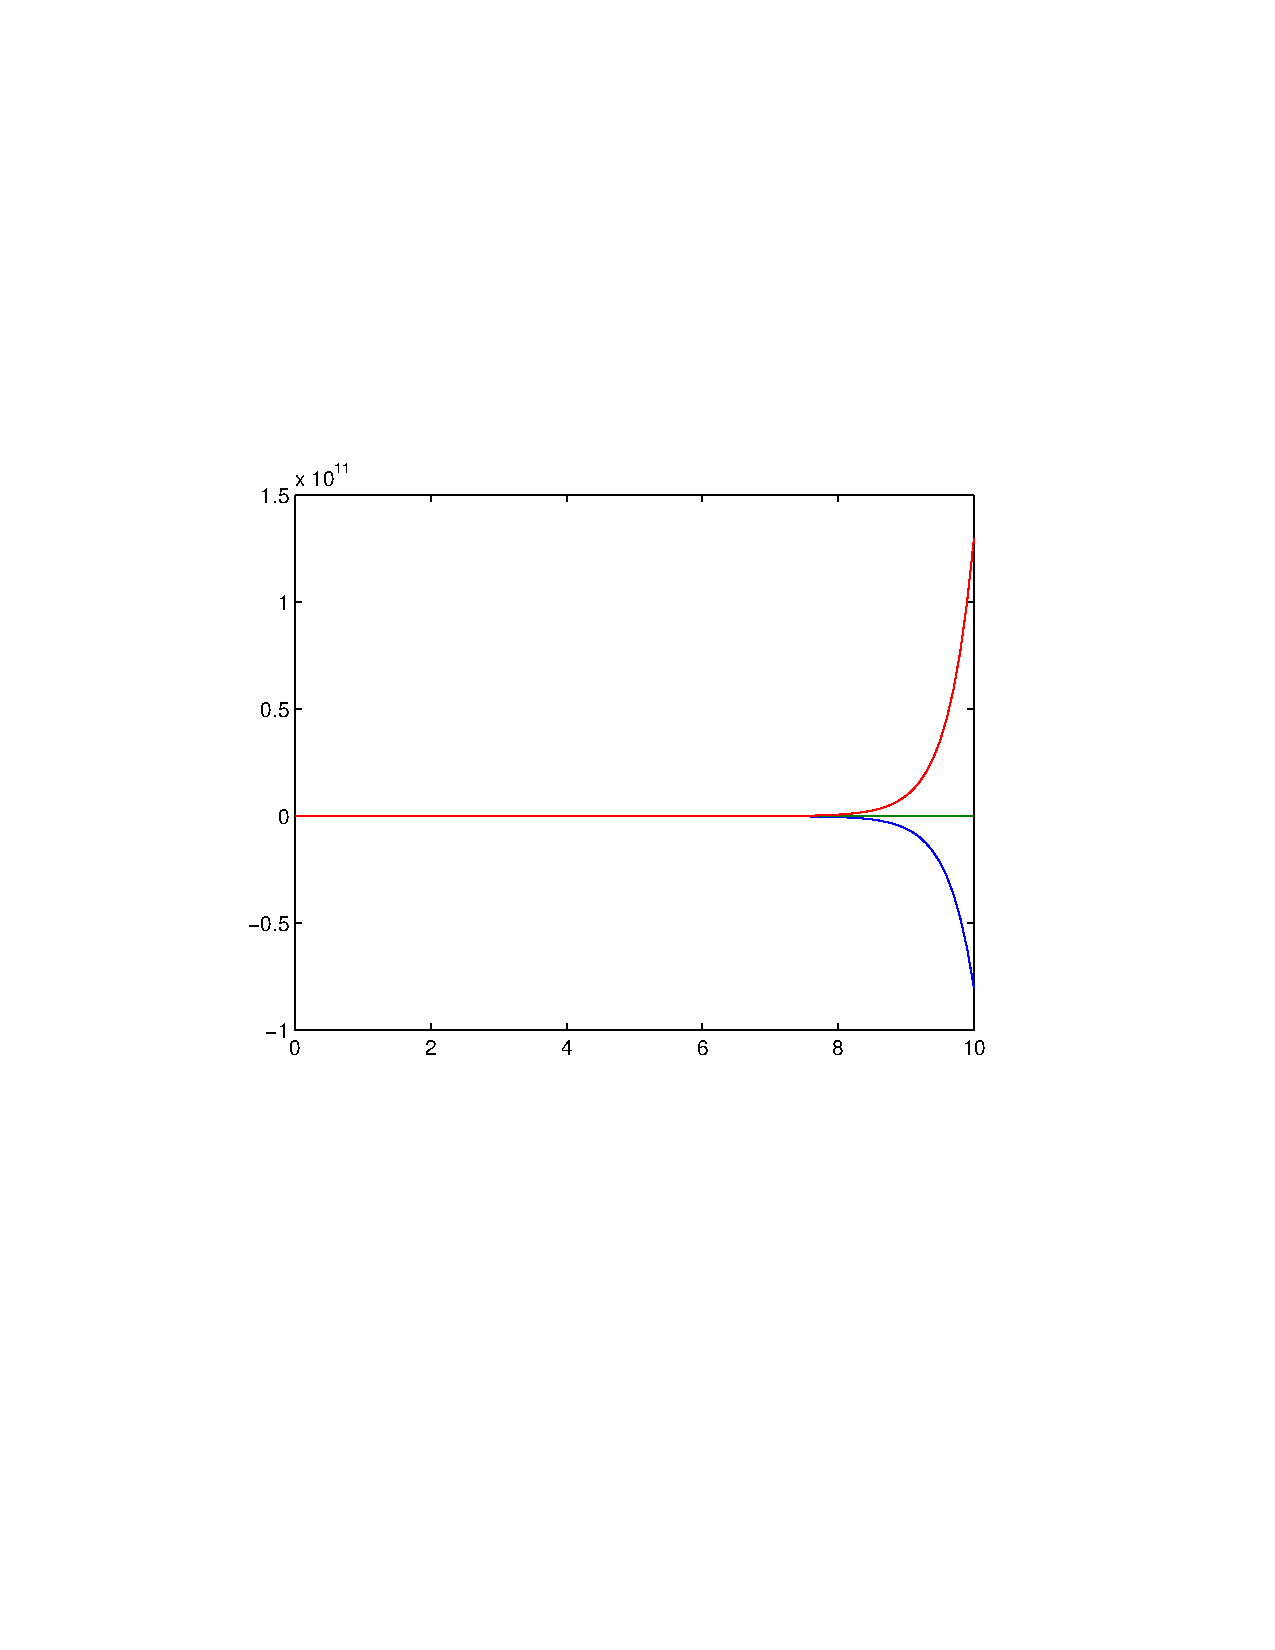
\includegraphics[width=\textwidth]{num2} 
\end{minipage}
\end{figure}

\section*{第三题}
状态方程的能空检验矩阵$Qc=\left(\begin{array}{ccc} B & AB & A^{2}B \end{array}\right)$ \\
$A= \left(\begin{array}{ccc} 1 & 0 & -1\\ 0 & -2 & 0\\ -1 & 0 & 2 \end{array}\right) $,
$AB=  \left(\begin{array}{c} -1\\ 0\\ 2 \end{array}\right) $,
$A^{2}B=  \left(\begin{array}{c} -3\\ 0\\ 5 \end{array}\right) $ \\
\mbox{所以 }$Qc= \left(\begin{array}{ccc} 0 & -1 & -3\\ 0 & 0 & 0\\ 1 & 2 & 5 \end{array}\right) $
\\可知该矩阵的佚为2,小于3,所以状态不完全能控\\
\noindent\\
状态方程的能观矩阵$Qo=\left(\begin{array}{ccc} C & CA & CA^{2} \end{array}\right) $
\\ $C= \left(\begin{array}{ccc} 1 & 0 & 0 \end{array}\right)$, 
$CA=\left(\begin{array}{ccc} 1 & 0 & -1 \end{array}\right)$,
$CA^{2}=\left(\begin{array}{ccc} 2 & 0 & -3 \end{array}\right)$ \\
\mbox{所以 }$Qo=\left(\begin{array}{ccc} 1 & 0 & 0\\ 1 & 0 & -1\\ 2 & 0 & -3 \end{array}\right)$
\\可知该矩阵的佚为2,小于3,所以状态不完全能观

\begin{verbatim}[matlab]
A=[1 0 -1; 0 -2 0; -1 0 2]; B=[0; 0; 1]; %输入系统状态方程
Qc=ctrb(A,B) %求系统能控性矩阵
rank(Qc) %求系统能控性矩阵的佚
ans = 2 %能控性矩阵的佚为2,所以系统不能控
 
A=[1 0 -1; 0 -2 0; -1 0 2]; C=[1 0 0] %输入系统状态方程;   
Qo=obsv(A,C)  %求系统能观性矩阵
rank(Qo) %求系统能控性矩阵的佚
ans = 2 %能观性矩阵的佚为2,所以系统不能观
\end{verbatim}
\section*{第四题}
欲使连续系统稳定,必须使特征方程 $|sI-A|=0$ 的根,亦即矩阵A的特征值,全部位于s平面的左半开平面上。\\
系统矩阵A为非奇异线性定常系统,$x_{e}=0$即原点,是系统的唯一平衡状态,其稳定性可由劳斯判据得到。\\
已知$|sI-A|=s^3 - s^2 - 5\, s + 2 =0 $ \\
列出如下劳斯表,由劳斯稳定判据可知,系统有两个正实根,即在该平衡点不稳定。
\begin{table*}[!h]
\centering
\begin{tabular}{c  c  c}  
$s^{3}$ & 1 & -5 \\ 
$s^{2}$ & -1 & 2 \\ 
$s^{1}$ & -3 & \\ 
$s^{0}$ & 2 & 
\end{tabular}
\end{table*}

\begin{verbatim}[matlab] 
det(s*eye(3)-A) = s^3 - s^2 - 5*s + 2 %求特征方程
solve(s^3 - s^2 - 5*s + 2) %求特征方程解 
ans =
              -2
 5^(1/2)/2 + 3/2=2.618
 3/2 - 5^(1/2)/2=0.382
可知系统有两个解在s平面的右半开平面上,该平衡点不稳定
\end{verbatim}

\section*{第五题}
\emph{能控性分解}\\
如上已知系统能控矩阵秩为2,小于3,故系统不完全能控。\\
$$Qc= \left(\begin{array}{ccc} 0 & -1 & -3\\ 0 & 0 & 0\\ 1 & 2 & 5 \end{array}\right) $$
\mbox{取Qc中线性独立的两列向量,这里取第一、二列,再补充一个与其他列向量无关的列向量 }$\left(\begin{array}{c} 0\\ 1\\ 0 \end{array}\right)$ \\
\mbox{可得到 }$Pc^{-1}=\left(\begin{array}{ccc} 0 & -1 & 0\\ 0 & 0 & 1\\ 1 & 2 & 0 \end{array}\right)$,$Pc=\left(\begin{array}{ccc} 2 & 0 & 1\\ -1 & 0 & 0\\ 0 & 1 & 0 \end{array}\right)$ \\
\mbox{则 }$ \bar{A} =P_{c}AP_{c}^{-1}= \left(\begin{array}{ccc} 0 & -1 & 0\\ 1 & 3 & 0\\ 0 & 0 & -2 \end{array}\right)$,
$ \bar{B} =P_{c}B=\left(\begin{array}{c} 1\\ 0\\ 0 \end{array}\right)$,
$ \bar{C} =CP_{c}^{-1}=\left(\begin{array}{ccc} 0 & -1 & 0 \end{array}\right)$
\noindent \\
能控子系统方程为
\begin{align*}
\dot{\bar{x}}_{c} &=  \left(\begin{array}{cc} 0 & -1\\ 1 & 3 \end{array}\right)x_{c}+\left(\begin{array}{c} 1\\ 0 \end{array}\right)u \\ 
y_{1} &= \left(\begin{array}{cc} 0 & -1 \end{array}\right)\bar{x}_{c}
\end{align*}
不能控子系统动态方程为
\begin{align*}
\dot{\bar{x}}_{\bar{c}} &= -2\bar{x}_{\bar{c}} \\
y_{2} &= 0
\end{align*}
\emph{能观性分解}\\
如上已知系统能观矩阵秩为2,小于3,故系统不完全能观。\\
$$ Q_{o}= \left(\begin{array}{ccc} 1 & 0 & 0\\ 1 & 0 & -1\\ 2 & 0 & -3 \end{array}\right)$$ \\
取$Q_{o}$中线性独立的两行向量,这里取第一、二行,再补充一个与其他行向量无关的行向量 $\left(\begin{array}{ccc} 0 & 1 & 0 \end{array}\right)$ \\
可得到$ P_{o}= \left(\begin{array}{ccc} 1 & 0 & 0\\ 1 & 0 & -1\\ 0 & 1 & 0 \end{array}\right), P_{o}^{-1}=\left(\begin{array}{ccc} 1 & 0 & 0\\ 0 & 0 & 1\\ 1 & -1 & 0 \end{array}\right)$ \\
则$ \bar{A}=P_{o}AP_{o}^{-1}= \left(\begin{array}{ccc} 0 & 1 & 0\\ -1 & 3 & 0\\ 0 & 0 & -2 \end{array}\right),
\bar{B}=P_{o}B= \left(\begin{array}{c} 0\\ -1\\ 0 \end{array}\right),
\bar{C}=CP_{o}^{-1}= \left(\begin{array}{ccc} 1 & 0 & 0 \end{array}\right)$ \\
能观子系统方程为\\
\begin{align*}
\dot{\bar{x}}_{o} &= \left(\begin{array}{cc} 0 & 1\\ -1 & 3 \end{array}\right)\bar{x}_{o}+\left(\begin{array}{c} 0\\ -1 \end{array}\right)u \\
y_1 &= \left(\begin{array}{cc} 1 & 0 \end{array}\right)\bar{x}_o
\end{align*}
不能观子系统方程为\\
\begin{align*}
\dot{\bar{x}}_{\bar{o}} &= -2\bar{x}_o \\
y_2 &= 0
\end{align*}
\begin{verbatim}[matlab验证]
能控性分解
A=[1 0 -1; 0 -2 0; -1 0 2]; B=[0; 0; 1]; C=[1 0 0];  %输入系统状态方程
Qc=ctrb(A,B) %求系统能控性矩阵
rank(Qc) = 2 %求系统能控性矩阵的佚  
能控性矩阵的佚为2,所以系统不完全能控,可以按能控性分解
[Ac, Bc, Cc, T, K]=ctrbf(A, B,C)
Ac =
    -2     0     0
     0     1     1
     0     1     2
Bc =
     0
     0
     1
Cc =
     0    -1     0
T =
     0     1     0
    -1     0     0
     0     0     1
K =
     1     1     0

能观性分解
Qo=obsv(A,C)  %求系统能观性矩阵   
rank(Qo) = 2 %求系统能控性矩阵的佚
能观性矩阵的佚为2,所以系统不完全能观,可以按能观性分解
[Ao, Bo, Co, T, K]=obsvf(A, B,C)
Ao =
    -2     0     0
     0     2     1
     0     1     1
Bo =
     0
    -1
     0
Co =
     0     0     1
T =
     0     1     0
     0     0    -1
     1     0     0
K =
     1     1     0     
\end{verbatim}
\section*{第六题}
已知$A=\left(\begin{array}{ccc} 1 & 0 & -1\\ 0 & -2 & 0\\ -1 & 0 & 2 \end{array}\right)$, 第二题已经求出矩阵A的特征值为$ -2, 0.382, 2.618$ \\
系统有两个特征值为正,故系统不稳定,由第五题可知,系统不能控。不能控子系统特征值为-2,符合可镇定条件。\mbox{故原系统可用状态反馈实现镇定,镇定后的极点设为 }$ -1,-2,-3 $。 \\
设状态反馈矩阵为$K=\left(\begin{array}{ccc} k_0 & k_1 & k_2 \end{array}\right)$ \\
$$ A-BK=\left(\begin{array}{ccc} 1 & 0 & -1\\ 0 & -2 & 0\\ -1 & 0 & 2 \end{array}\right)-
\left(\begin{array}{c} 0\\ 0\\ 1.0 \end{array}\right)
\left(\begin{array}{ccc} k_0 & k_1 & k_2 \end{array}\right)=\left(\begin{array}{ccc} 1 & 0 & -1\\ 0 & -2 & 0\\  - k_0 - 1 & -k_1 & 2 - k_2 \end{array}\right) $$
则状态反馈系统特征方程为
$$ \left|sI-(A-BK)\right|= s^3+(k_2-1)s^2+(k_2-k_0-5)s+2-2k_2-2k_0$$ 
期望闭环极点为$-1,-2,-3$,则对应的系统特征方程为
$$ (s+2)(s+1)(s+3)=s^3 + 6\, s^2 + 11\, s + 6 $$ 
比较对应项系数,可得 
\begin{align*}
k_2-1 &= 6 \\
k_2-5-k_0 &=11 \\
2-2k_2-2k_0 &=6
\end{align*}
结果为$k_0=-9,k_1=0,k_2=7$, 则$ k=\left(\begin{array}{ccc} -9 & 0 & 7 \end{array}\right) $ \\
\mbox{所以 }$\dot{x}=(A-BK)x+BV=\left(\begin{array}{ccc} 1 & 0 & -1\\ 0 & -2 & 0\\ 8 & 0 & -5 \end{array}\right)x+\left(\begin{array}{c} 0\\ 0\\ 1 \end{array}\right)V$ \\
计算转移矩阵的方法同第二题,同理可得\\
\mbox{状态转移矩阵 }$ \Phi(t)=e^{(A-BK)t}=\left(\begin{array}{ccc} 2\, \mathrm{e}^{- t} - \mathrm{e}^{- 3\, t} & 0 & \frac{\mathrm{e}^{- 3\, t}}{2} - \frac{\mathrm{e}^{- t}}{2}\\ 0 & \mathrm{e}^{- 2\, t} & 0\\ 4\, \mathrm{e}^{- t} - 4\, \mathrm{e}^{- 3\, t} & 0 & 2\, \mathrm{e}^{- 3\, t} - \mathrm{e}^{- t} \end{array}\right) $\\
\mbox{已知 }$x(t)=\Phi(t)x(0)+\int_{0}^{t}\Phi(t-\tau)Bu(\tau)d\tau $ \\
\mbox{其中 }$\Phi(t)x(0)=\left(\begin{array}{c} \frac{3\, \mathrm{e}^{- t}}{2} - \frac{\mathrm{e}^{- 3\, t}}{2}\\ 2\, \mathrm{e}^{- 2\, t}\\ 3\, \mathrm{e}^{- t} - 2\, \mathrm{e}^{- 3\, t} \end{array}\right),
\int_{0}^{t}\Phi(t-\tau)Bu(\tau)d\tau=\left(\begin{array}{c} \frac{\mathrm{e}^{- t}}{2} - \frac{\mathrm{e}^{- 3\, t}}{6} - \frac{1}{3}\\ 0\\ \mathrm{e}^{- t} - \frac{2\, \mathrm{e}^{- 3\, t}}{3} - \frac{1}{3} \end{array}\right) $ \\
\mbox{所以 }$x(t)=\left(\begin{array}{c} 2\, \mathrm{e}^{- t} - \frac{2\, \mathrm{e}^{- 3\, t}}{3} - \frac{1}{3}\\ 2\, \mathrm{e}^{- 2\, t}\\ 4\, \mathrm{e}^{- t} - \frac{8\, \mathrm{e}^{- 3\, t}}{3} - \frac{1}{3} \end{array}\right)$ \\
\begin{figure}[htbp]
\begin{minipage}[c]{0.45\textwidth}
\begin{verbatim}[matlab验证]
syms t,tao %定义时间变量t, tao为符号
A=[1 0 -1; 0 -2 0; -1 0 2]; k=[-9 0 7];
B=[0; 0; 1]; x0=[1; 2; 1] %输入系统状态方程和初始值
xt=expm((A-B*K)*t)*x0+int(expm(A-B*K)*(t-tao)*B,tao,0,t) %求非齐次解
绘出单位阶跃响应的系统状态轨迹图
t=0:0.1:10
plot(t,xt(1), t,xt(2), t,xt(3))
\end{verbatim}
\end{minipage}
\begin{minipage}[c]{0.5\textwidth}
\caption{单位阶跃响应的系统状态轨迹图}
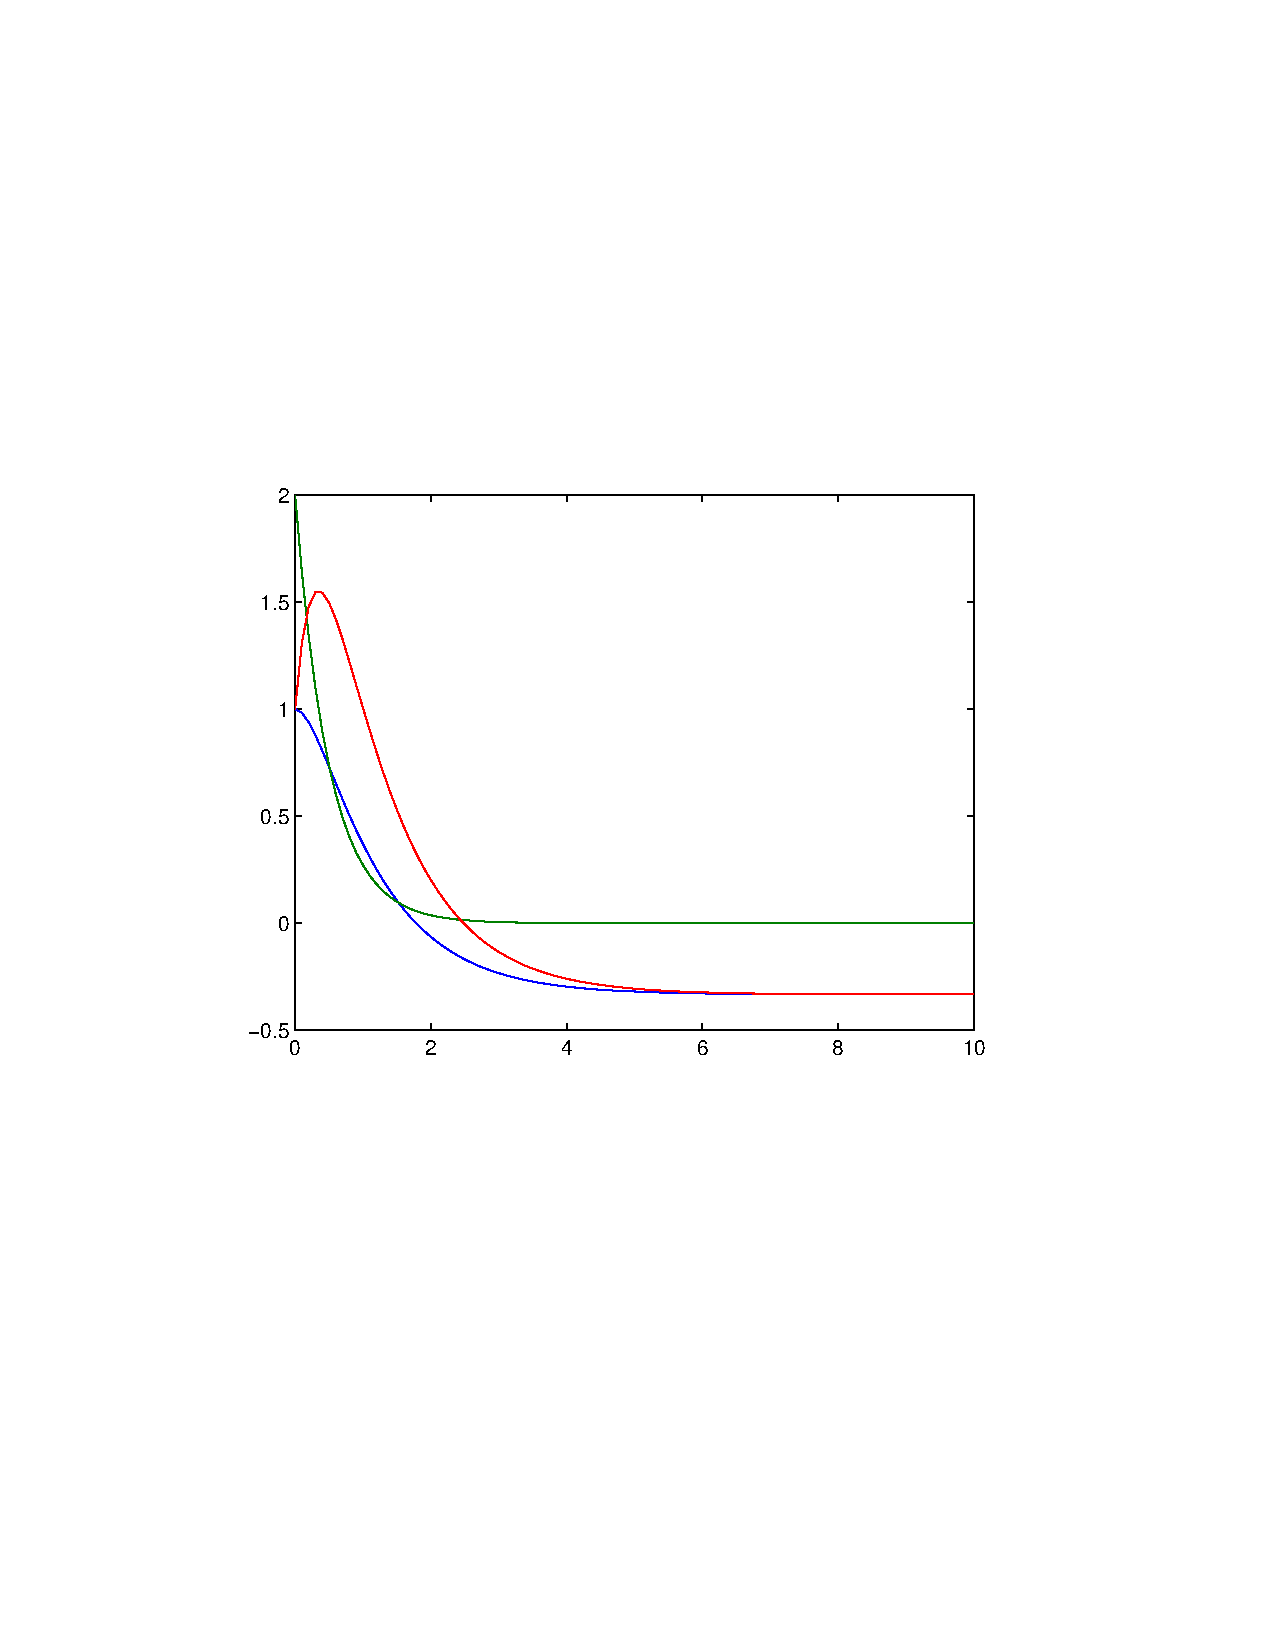
\includegraphics[width=\textwidth]{num6} 
\end{minipage}
\end{figure}
\end{document}
